\section{Comparison: Measurement and Theoretical Values}\label{sec:meas_vs_theory}

The aim of this section is to compare the measured polar response of the speaker array with values estimated using the analytical model with and without pressure correction and the \gls{fdtd} simulation. This section will not evaluate the cost filter. Therefore the results are presented as a relative \gls{spl}, where \SI{0}{\decibel} typically is reached in front of the array. This is achieved by norming the pressure along the circumference at each given frequency to the maximum pressure at that particular frequency.
%All polar plots in \autoref{the_simulation_result} are converted to relative value, where the maximum value is the reference. 
The reason to use the maximum value and not the pressure on main axis of the speaker array is, that the measurement might suffer from misalignment, which leads to the highest pressure not being exactly on the main axis. 
When describing graphs, often the term of \textit{attenuation} will be used. This term shall be defined as the additive inverse of the normed \gls{spl}, meaning that a bigger attenuation corresponds to a smaller relative pressure level.\\
The performance of the cost filter and therefore the absolute \gls{spl} will be evaluated in \autoref{sec:beamforming_array_spl}.\\

For a frequency of \SI{60}{\hertz}, results are shown in \autoref{fig:60_hz_polar_result}. The directional characteristics estimate calculated with the analytical model in its unaugmented form, based on only pulsating spheres, and the augmented analytical model with a correction table, are widely similar. The augmented model is a little more ``optimistic'', predicting a slightly smaller lobe width and lower pressure \SI{180}{\degree}. There is an anomaly in the augmented graph at approx. \SI{2}{\degree}, where there is a spike in the pressure curve. This is due to some imprecision or glitch in the measurement (\autoref{ax:directional_2}), that the correction table is based upon. The predicted directional characteristics derived from \gls{fdtd}-simulation are very similar to those based on the unaugmented analytical model at angles up to \SI{\pm 120}{\degree}. However, it shows significantly less attenuation, where both analytical models have spikes at \SI{\pm 135}{\degree}. At the back lobe at \SI{180}{\degree}, the beamforming is estimated to be slightly less effective (approx. \SI{-15}{\decibel} \gls{fdtd} vs. approx \SI{-15.5}{\decibel} analytical) then the unaugmented analytical model predicts. The measured directional characteristics match up quite well with the \gls{fdtd}-based and the unaugmented analytical estimates for angles close to \SI{0}{\degree}. As the angles progress towards the back, more deviation occurs. The beamforming performance is worse then estimated, especially at at \SI{\pm 135}{\degree}, where, instead of spiking, the attenuation only gradually increases to approx. \SI{-15}{\decibel}. Still, this a larger pressure reduction then at \SI{180}{\degree}, which means the array has a supercardiod directional characterstic at this frequency. At an angle of \SI{180}{\degree}, a pressure reduction of \SI{12}{\decibel} compared to the main axis is achieved. At approx. \SI{-132}{\degree}, there is an anomaly in the measured graph. This is likely to be due to a glitch in the measurement routine. Apart from this, the measured curve is approximately symmetrical.\\
At a frequency of \SI{60}{\hertz}, the \gls{fdtd}-based estimate of the directional characteristics predicts measured behaviour of the speaker array most accurately.
\begin{figure}[H]
	\centering
	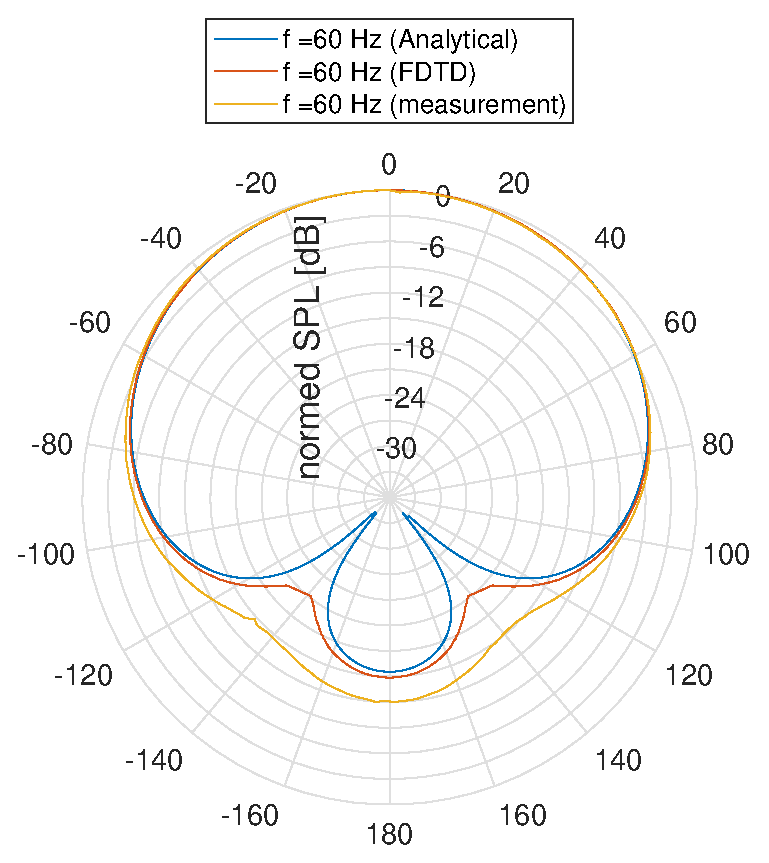
\includegraphics[width=0.85\textwidth]{60_hz_polar_result.eps}
	\caption{Directional characteristics, \SI{60}{\hertz}}
		\label{fig:60_hz_polar_result}
\end{figure}
For a frequency of \SI{100}{\hertz}, results are shown in \autoref{fig:100_hz_polar_result}. Just like at \SI{60}{\hertz}, the augmented analytical model leads to a similar graph to the unaugmented analytical model, while being slightly more optimistic. The graph corresponding to the \gls{fdtd}-based approach predicts slightly less attenuation compared to the analytical models everywhere, except around \SI{\pm 135}{degree}, where it predicts significantly less attenuation reduction. The measured graph starts deviating from the predicted characteristic close to \SI{0}{\degree} stronger then it did at \SI{60}{\hertz}. There is less attenuation than predicted by all of the models up to angles of approx. \SI{\pm 155}{\degree}. The calculated estimates all show supercardiod characteristics. Towards the back direction (\SI{180}{\degree}) they predict a lobe, where the estimates range from approx. \SI{14.5}{\decibel} (\gls{fdtd}) to approx. \SI{15.5}{\decibel} attenuation. The measurement result is actually better then this with an attenuation of approx. \SI{17.5}{\decibel} at \SI{180}{\degree}. The shape of the measured graph indicates more of a non-hypercardiod but cardiod characteristic, meaning there is no back lobe. However, there is some asymmetry in the graph. The maximum attenuation of \SI{18}{\decibel} is actually achieved around \SI{-160}{\degree}.\\
It is hard to declare a winner for \SI{100}{\hertz}, because all estimation approaches actually show a significantly different shape compared to the measurement results. However, the \gls{fdtd}-based approach appears to lead to a smaller error compared to both analytically based approaches. 
\begin{figure}[H]
	\centering
	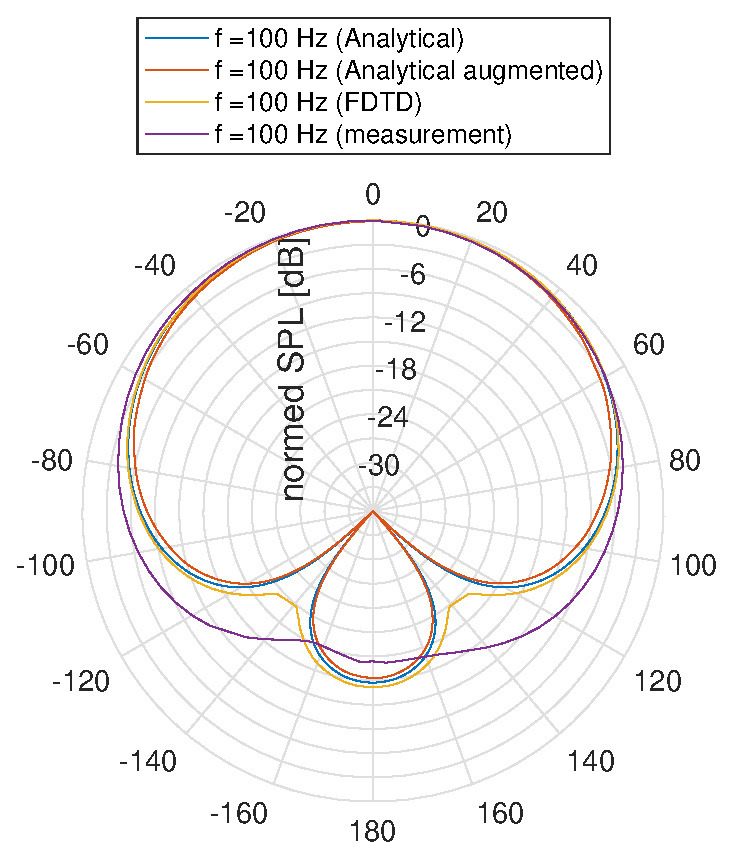
\includegraphics[width=0.85\textwidth]{100_hz_polar_result.eps}
	\caption{Directional characteristics, \SI{100}{\hertz}}
		\label{fig:100_hz_polar_result}
\end{figure}
For a frequency of \SI{150}{\hertz}, results are shown in \autoref{fig:150_hz_polar_result}.
All three calculated estimation approaches behave very similarly to what has been described for the frequencies of \SI{60}{\hertz} and \SI{100}{\hertz}. Opposed to that, the measured characteristics change their shape significantly compared to \SI{100}{\hertz}. The graph is now clearly supercardiod and matches the estimates qualitatively but not quantitatively.
Close to \SI{0}{\degree}, the measured graph matches the unaugmented analytical model and the \gls{fdtd}-based approach well. The attenuation becomes increasingly smaller than predicted for larger angles up to approx. \SI{\pm 130}{\degree}. There are two distinct spikes in the curve, one at approx. \SI{-150}{\degree} that corresponds to an attenuation bigger than \SI{40}{\decibel} and the other one at approx. \SI{150}{\degree} with less attenuation. The back lobe is narrower than predicted. The attenuation at \SI{180}{\degree} is approx. \SI{15.5}{\decibel}, which matches the value predicted by the augmented analytical model almost exactly.\\
At \SI{150}{\hertz} the analytical models appears to deliver the closer resemblies of the measured graph, because unlike the \gls{fdtd}-based approach they correctly predict spikes in the attenuation graph. The unaugmented analytical model is closer to the measured data for the front lobe, while the augmented analytical model is more accurate for the back lobe. The spikes in the measured graph appear closer to \SI{180}{\degree} than predicted.
\begin{figure}[H]
	\centering
	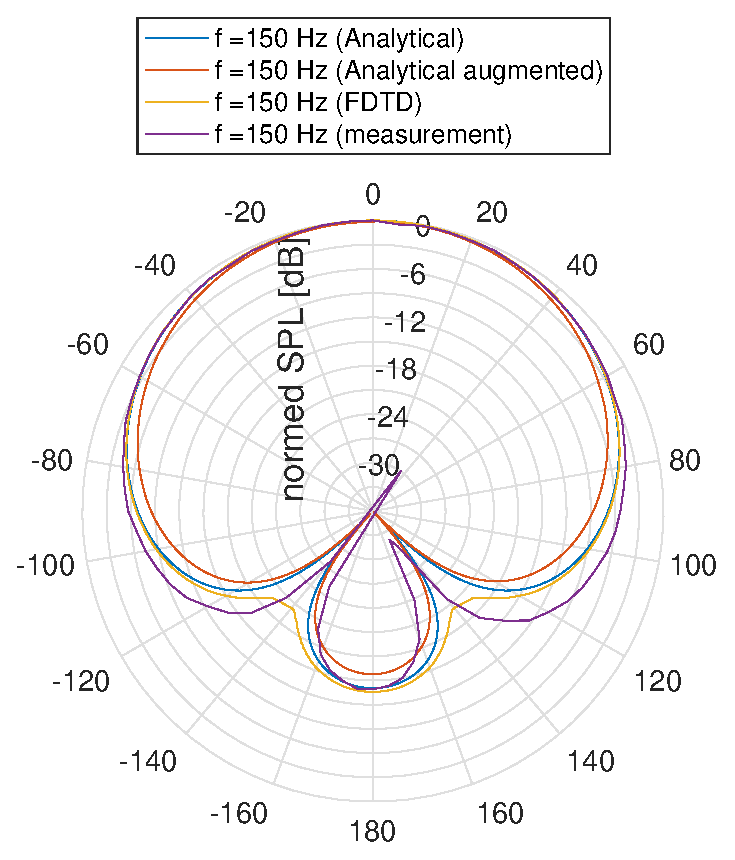
\includegraphics[width=0.85\textwidth]{150_hz_polar_result.eps}
	\caption{Directional characteristics, \SI{150}{\hertz}}
		\label{fig:150_hz_polar_result}
\end{figure}
For a frequency of \SI{200}{\hertz}, results are shown in \autoref{fig:200_hz_polar_result}. Again the calculated predictions show a similar behaviour to what has been described above. It should be noticed, that the augmented analytical model tends to have increasingly ``optimistic'' results compared to the unaugmented model towards higher frequencies, because it takes into account that the loudspeakers in the array have a tendency to behave not perfectly omnidirectional at higher frequencies. This however is not confirmed by the measured graph, which shows some significant asymmetry. For positive angles (right side), the measured graph is very close to what is predicted by the \gls{fdtd}-based approach. For negative angles (left side), the measured graph behaves more like it did at \SI{150}{\hertz}, which means, the attenuation is overestimated by the models for the main lobe and there is a huge spike at approx. \SI{-150}{\degree}, which is closer to \SI{180}{\degree} than predicted. The attenuation at \SI{180}{\degree} is approx. \SI{12.5}{\decibel} and matches the \gls{fdtd}-based approach very closely. However, the ``tip'' of the back lobe seems to be at \SI{170}{\degree}, where the attenuation is closer to \SI{12}{\decibel}. Overall, the \gls{fdtd}-based approach delivers the closest prediction to the measured behaviour at \SI{200}{\hertz}. If the asymmetry of the measured graph is due to some imprecisions in the loudspeaker placement, it might as well be, that, for an array, that is set up more precisly, the measured characteristics might behave like an average of the two sides that are seen in this measurement. This might actually make the unaugmented analytical model the most accurate representation.
%It again shows a supercardiod characteristic and matches the predictions well near \SI{0}{\degree} but shows less attenuation towards angles that are further away from the main axis. Similar to \autoref{fig:150_hz_polar_result} at \SI{200}{\hertz} the spikes in the measured graph around approx. \SI{\pm 140}{\degree} are asymmetrical, with the one at approx. \SI{-140}{\degree} peaking at a larger attenuation then the one at approx. \SI{140}{\degree}. The shape of the graph is also asymmetric in the aspect that back lobe is wider towards the positive angles and the smallest attenuation of the back lobe is not at \SI{180}{\degree}, but at \SI{175}{\degree}.
 \begin{figure}[H]
	\centering
	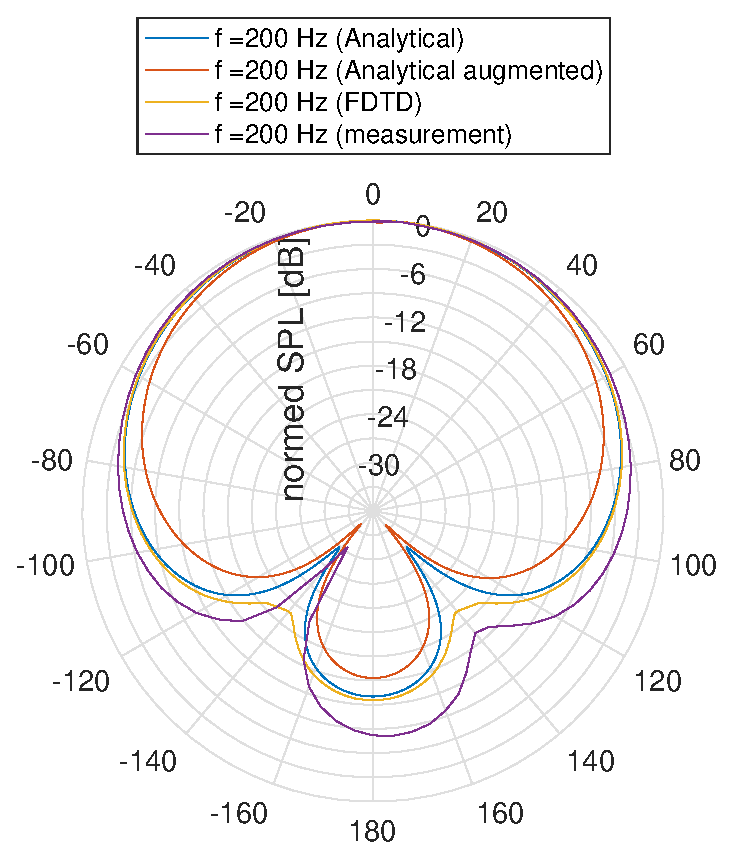
\includegraphics[width=0.85\textwidth]{200_hz_polar_result.eps}
	\caption{Directional characteristics, \SI{200}{\hertz}}
		\label{fig:200_hz_polar_result}
\end{figure}
For a frequency of \SI{250}{\hertz}, results are shown in \autoref{fig:250_hz_polar_result}.
Like at \SI{200}{\hertz}, the measured graph is asymmetric. For positive angles up to approx. \SI{95}{\degree}, the measurement matches the attenuation predicted by the augmented analytical model. Closer to \SI{180}{\degree} the measured attenuation is closer to the prediction by the \gls{fdtd}-based approach, including a notch instead of a peak at approx. \SI{140}{\degree}. For negative angles, the measured graph is closest to the ones corresponding to the unaugmented analytical model and the \gls{fdtd}-based approach. Like on the right side, there is more of a notch instead of a spike in attenuation at approx. \SI{-150}{\degree}. This means, like at most other frequencies, it occurs closer to \SI{180}{\degree} than predicted. The measured attenuation at \SI{180}{\degree} is approx. \SI{12.5}{\decibel}, exceeds the predictions from the unaugmented analytical and \gls{fdtd}-based approach by approx. \SI{0.5}{\decibel} but is significantly less then the \SI{15}{\decibel} predicted by the augmented analytical model.
 \begin{figure}[H]
	\centering
	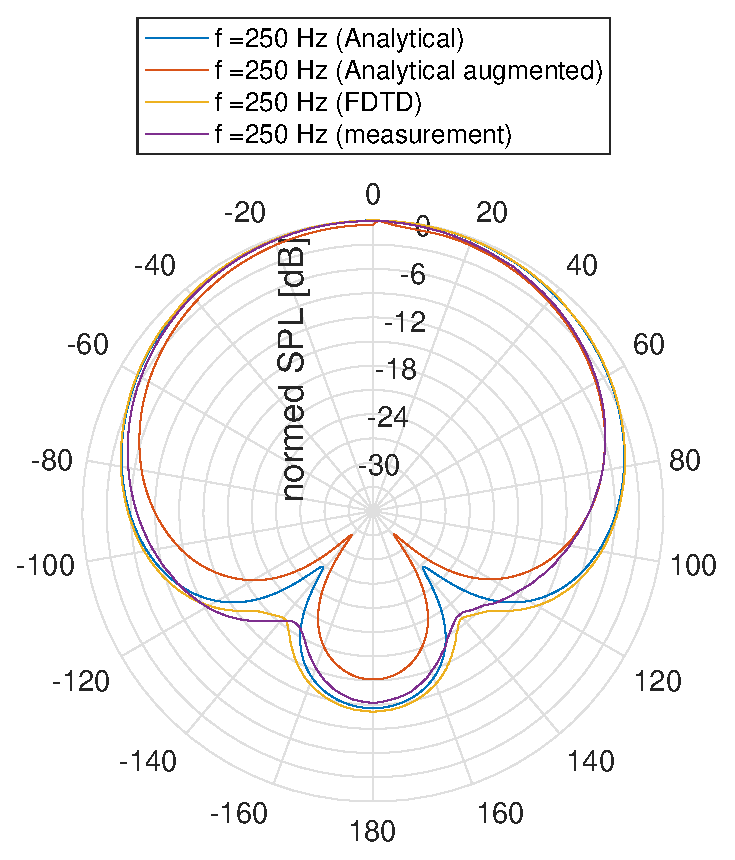
\includegraphics[width=0.85\textwidth]{250_hz_polar_result.eps}
	\caption{Directional characteristics, \SI{250}{\hertz}}
		\label{fig:250_hz_polar_result}
\end{figure}
For a frequency of \SI{300}{\hertz}, results are shown in \autoref{fig:300_hz_polar_result}. The measured graph is slightly asymmetrical. Up to \SI{\pm 100}{\degree}, the measured attenuation matches the attenuation predicted by augmented analytical model quite well. The notches in the measured graph occur significantly closer to \SI{180}{\degree} than prediced. The measured attenuation is smaller than predicted by the augmented analytical model up to approx. \SI{150}{\degree} and it is bigger than predicted for any angle closer to \SI{180}{\degree}. The back lobe is smaller than predicted and the attenuation at \SI{180}{\degree} is approx. \SI{18}{\decibel}, which is a larger attenuation than predicted by any of the models. Even though the shape of the measured graph is not closely matched by any of the models, the augemented analytical approach delivers a reasonably accurate estimate up to \SI{\pm 100}{\degree}.
 \begin{figure}[H]
	\centering
	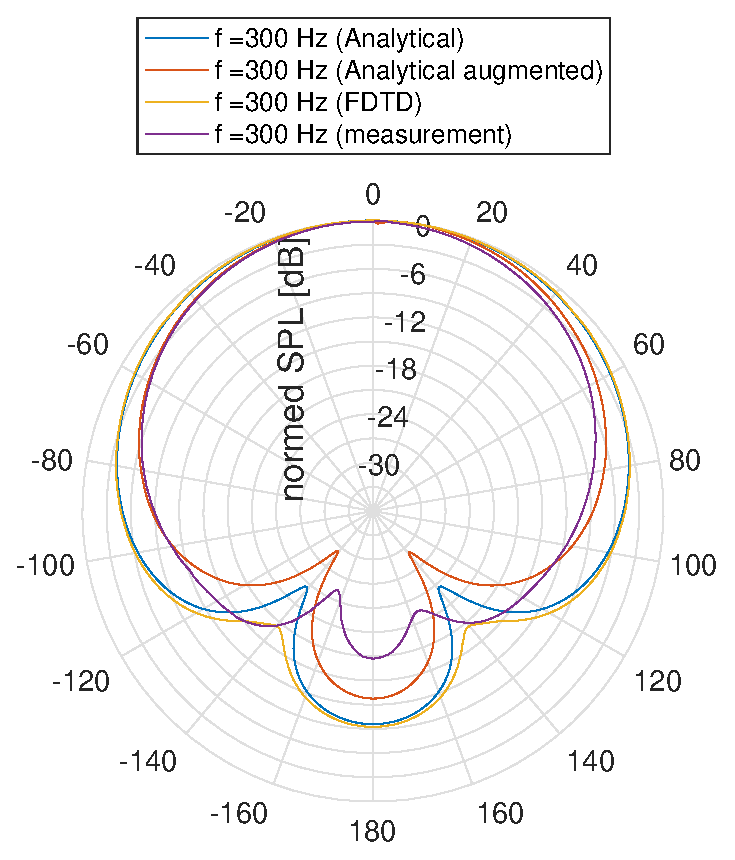
\includegraphics[width=0.85\textwidth]{300_hz_polar_result.eps}
	\caption{Directional characteristics, \SI{300}{\hertz}}
		\label{fig:300_hz_polar_result}
\end{figure}


\section{Conclusion on the Comparison}\label{meas_vs_theory_conclusion}
It can be concluded, that except for a frequency of \SI{100}{\hertz} (\autoref{fig:100_hz_polar_result}), at all frequencies that have been contemplated in \autoref{sec:meas_vs_theory}, the measured graphs have a supercardiod shape, like predicted in all of the models. As to which of the three approaches delivers the closest prediction of the measured results, there is no clear winner. For the lowest frequencies (\SI{60}{\hertz}, \SI{100}{\hertz}), the \gls{fdtd}-based predictions appear to be most accurate. At the frequencies (\SI{150}{\hertz}, \SI{200}{\hertz}), at which big spikes in the graphs occur around \SI{\pm 145}{\degree}, the unaugmented analytical model gives good predictions of the quality of the measured graphs, but it shows some weaknesses when it comes to quantity. At the highest of frequencies (\SI{250}{\hertz}, \SI{300}{\hertz}), the augmented analytical model is in advantage close to the main axis of the array, but it fails to predict the behaviour in the back properly. Of course, some of the deviation might be due to the unknown influence of the array on the positions of the acoustic centers, that possibly be taken into account, if a recursive parameter optimization would have taken place (see \autoref{sec:ideal_approach}). This would have also affected the correction tables for the augmented model. From the knowledge that is available right now, it seems like, depending on the intended application, for frequencies up to \SI{200}{\hertz} changing between the unaugmented analytical approach and the \gls{fdtd}-based approach only has little effect on the quality of the estimates. For computational efficiency reasons, the analytical approach might be favorable in many applications. It also shows, that the analytical model, that has also been used to determine fitness values in the optimization of \gls{sp}-parameters, is a reasonably representative way of assessing the performance of the solutions in the \gls{ga}. More research is required, in order to draw a meaningful conclusion, on whether the concept of the augmented analytical model can be perfected to deliver accurate predictions over the whole frequency range, that this project has investigated.